%chktex-file 36
%chktex-file 23
%chktex-file 10
%chktex-file 17
%chktex-file 9
\documentclass[computationalMathematics.tex]{subfiles}

\begin{document}

%%%%%%%%%%%%%%~~~~~~~~~~~~~~~~~~~~~~~~~~~~~~~~~~~~~~~~%%%%%%%%%%%%%%%
\section{3rd of October 2018 --- A. Frangioni}
%%%%%%%%%%%%%%~~~~~~~~~~~~~~~~~~~~~~~~~~~~~~~~~~~~~~~~%%%%%%%%%%%%%%%
\begin{example}[On derivatives]
Let $f:\R^2 \to \R$ such that $f(x, y) = x^2 e^y$. Compute the partial derivatives.

$\frac{\partial f}{\partial x} = 2x e^y $i; $\frac{\partial f}{\partial y} = x^2 e^y $

$\frac{\partial f}{\partial [0, 1]} = \lim\limits_{t \to 0} \frac{f(x + t_1, y + t_0)}{t} =  \lim\limits_{t \to 0} \frac{f(x + t, y)}{t}$, which is equivalent to the derivative of the second component.

Conversely, $\frac{\partial f}{\partial [1, 0]}$ is equivalent to the derivative in the first component.
\end{example}
We have that the partial derivative on a certain direction $d$ is the scalar product between the gradient and the direction, formally

\[
  \frac{\partial f}{\partial d} = \ps{\begin{pmatrix}2x e^y\\ x^2 e^y\end{pmatrix}}{\begin{pmatrix} d_1\\ d_2 \end{pmatrix}}
\]

\begin{definition}[Vector-valued function]
  Let $f: \R^n \to \R^m$ is termed \textbf{vector-valued function}, where $f(x) =  [f_1(x),~f_2(x), \ldots,~f_m(x)]$.
\end{definition}

For such functions the computation of the derivative requires to specify not only the component, but also the index of the function.

\begin{definition}[Partial derivative for vector-valued functions]
Let $f: \R^n \to \R^m$, the partial derivative of the $j$-th function of the $i$-th component is
\[
   \frac{\partial f_{j}}{\partial x_i}(x) =
   \lim_{t \to 0} \frac{f_{j}(x_1, x_2, \ldots, x_{i-1}, \ldots, x_i + t, x_{i+1}, \ldots, x_n) - f_{j}(x)}{t}
\]
\end{definition}

\begin{definition}[Jacobian]
  Let $f: \R^n \to \R^m$ we call \textbf{Jacobian} the matrix of all its first-order partial derivatives.
\[
  Jf(x) =
  \begin{pmatrix}
    \frac{\partial f_1}{\partial x_1} & \cdots & \frac{\partial f_1}{\partial x_n}\\
    \vdots & \ddots & \vdots\\
    \frac{\partial f_m}{\partial x_1} & \cdots & \frac{\partial f_m}{\partial x_n}\\
  \end{pmatrix}
  =
  \begin{pmatrix}
    \nabla f_1(x)\\
    \nabla f_2(x)\\
    \vdots\\
    \nabla f_m(x)
  \end{pmatrix}
\]
\end{definition}

Notice that when the number of variables increases the first derivative is a vector of numbers, the second derivative contains $n^2$ numbers.

\begin{example}
Let $f:\R^2 \to \R$ such that $f(x, y) = x^2 e^y$. The gradient was computed above, resulting in
  
\[
  \nabla f(x)
  =
  \begin{pmatrix}
    \frac{\partial f}{\partial x}\\
    \frac{\partial f}{\partial y} 
  \end{pmatrix}
  =
  \begin{pmatrix}
    2x e^y\\
    x^2 e^y
  \end{pmatrix}
\]

Let us compute the second derivative of this function:
\[
  \nabla^2 f(x)
  =
  \begin{pmatrix}
    \frac{\partial^2 f}{\partial x \partial x} & \frac{\partial^2 f}{\partial y \partial x}\\

    \frac{\partial^2 f}{\partial x \partial  y} & \frac{\partial^2 f}{\partial y \partial y}\\

  \end{pmatrix}
  =
  \begin{pmatrix}
    2 e^y & 2x e^y\\
    2x e^y & x^2 e^y\\
  \end{pmatrix}
\]
\end{example}

\begin{definition}[Hessian]
  Let $f: \R^n \to \R^m$, we call \textbf{Hessian} of $f$
  \[
  \nabla^2 f(x) := J \nabla f(x) =
  \begin{pmatrix}
   \frac{\partial^2 f}{\partial x_1^2}(x) &
   \frac{\partial^2 f}{\partial x_2 \partial x_1}(x) & \cdots &
   \frac{\partial^2 f}{\partial x_n \partial x_1}(x)\\
   %
   \frac{\partial^2 f}{\partial x_1 \partial x_2}(x) &
   \frac{\partial^2 f}{\partial x_2^2}(x) & \cdots &
   \frac{\partial^2 f}{\partial x_n \partial x_2}(x) \\
   %
   \vdots & \vdots & \ddots & \vdots \\
   %
   \frac{\partial^2 f}{\partial x_1 \partial x_n}(x) &
   \frac{\partial^2 f}{\partial x_2 \partial x_n}(x) & \cdots &
   \frac{\partial^2 f}{\partial x_n^2}(x)
  \end{pmatrix}
\]
\end{definition}

The size of the matrix grows very rapidly with the number of derivatives that we make.

In optimization, we like to work with Hessians, but they need to be handled, because they are very large, hence a trade off is needed.

In most cases, the Hessian is symmetric, meaning that the order in which we derive is not relevant and this happens when $\exists \delta > 0$ s.t.~$\forall y \in \mathcal{B}(x, \delta)$ $\frac{\partial^2 f}{\partial x_j \partial x_i}(y)$ and  $\frac{\partial^2 f}{\partial x_i \partial x_j}(y)$ exist and $\frac{\partial^2 f}{\partial x_j \partial x_i}(y)$ and  $\frac{\partial^2 f}{\partial x_i \partial x_j}(y)$ are continuous at $x$.


\begin{definition}[$C^2$ functions]
  Let $f: \R^n \to \R^m$. We say that $f$ \textbf{belongs to $C^2$ class} iff $\nabla^2 f(x)$ is continuous.
\end{definition}

\begin{property}
Let $f: \R^n \to \R^m$ such that $f \in C^2$, then
\begin{itemize}
  \item $\nabla^2 f(x)$ symmetric
  \item $\nabla f(x)$ continuous
\end{itemize}
\end{property}

\begin{definition}[First order Taylor model]
Let $f : \R^n \to \R \in C^1$ in some $\mathcal{B}(x, \delta)$, we define the \textbf{first-order Taylor's formula}  $\forall y \in \mathcal{B}(x, \delta)~\exists ~ \alpha \in (0, 1)$ s.t.
\[
  f(y) = \ps{\nabla f(\alpha x + (1 - \alpha) y}) {y - x} + f(x)
\]
Intuitively, it is a linear approximation of the function $f$ in a neighbourhood of $x$. 

  Equivalently, we can write the so-called \textbf{remainder version of first-order Taylor formula} as

\[
  f(y) = \ps{\nabla f(x)}{y - x} + f(x)+ R(y - x)
\]
  where $\lim\limits_{h \to 0} \frac{R(h)}{\norm{h}} = 0$, in other words the error that we make is at most quadratic.
\end{definition}

Notice that this is a completely local thing, the furthest we get from $x$ the mor distant the function and the model are.

\begin{example}
Let $f:\R^2 \to \R$ such that $f(x, y) = x^2 e^y$. The gradient was computed above and now we have $f(1, 0) = 1$, $\nabla f(1, 0) = \begin{pmatrix}2\\1\end{pmatrix}$.

The linear model has the following shape $L_{(1, 0)} (x, y) = 1 + \ps{\begin{pmatrix}2\\ 1\end{pmatrix}}{\begin{pmatrix} x-1\\ y-0\end{pmatrix}} = -1 + 2x + y$.

And the quadratic model is 
  \begin{equation}
    \begin{split}
      Q_{[1, 0]} (x, y) &= -1 + 2x + y + \frac{1}{2} \cdot \begin{pmatrix}x-1 & y-0\end{pmatrix} \cdot \begin{pmatrix} 2 & 2\\ 2 & 1 \end{pmatrix} \cdot \begin{pmatrix} x-1 \\ y-0 \end{pmatrix}\\ 
      &= -1 +2x + y + \frac{1}{2} \cdot \begin{pmatrix} 2x -2 +2y, & 2x -2 +y \end{pmatrix} \cdot \begin{pmatrix} x-1\\ y-0\end{pmatrix}\\
      &= -1 + 2x + y + \frac{1}{2} \cdot (2x -2 + 2y) \cdot (x-1)  + (2x -x +y) \cdot y
    \end{split}
    \end{equation}
\end{example}

\begin{definition}[Second order Taylor model]
Let $f : \R^n \to \R \in C^1$ in some $\mathcal{B}(x, \delta)$, we define the \textbf{second-order Taylor's formula}  
\[
  f(y) = L_x(y) + \frac{1}{2} \tr{(y - x)} \nabla^2 f(x) (y - x) + R(y - x)
\]
  with $\lim\limits_{h \to 0} R(h) \norm{h}^2 = 0 \equiv$ the error is $O(\norm{y - x}^3) \equiv$ the remainder vanishes at least cubically.
\end{definition}

Notice that the $k$-th order Taylor expansion with $k$-th order derivatives, but $\nabla^k f(x)$ tensor of order $k \equiv n^k$ numbers.
Often $k > 2$ is unfeasible, so this approach cannot be followed.

\begin{proposition}
  Let $f : \R^n \to \R \in C^1$. If $f$ Lipschitz continuous on $S$, then $\sup \{\norm{\nabla f(x)}~:~x \in S\} \leq L$ ($\iff$, and $= L$ if $S$ convex).
\end{proposition}

Moreover, we can prove

\begin{proposition}
Let $f : \R^n \to \R \in C^1$. $f$ is Lipschitz continuous on $S$ iff $\nabla^2 f$ is bounded on $S$.

Equivalently, iff $\lambda_1(\nabla^2 f)$ is bounded.
\end{proposition}

\begin{proposition}
  Let $f : \R^n \to \R \in C^1$. If $\nabla f$ is Lipschitz continuous, then $f(y) \leq L_x(y) + \frac{L}{2} \norm{y - x}^2$.
\end{proposition}

The approximations are good because they give an hint about where the function is decreasing.
The limitation is that we cannot take too be steps, because the derivative information is accurate only locally.

Moreover, we need to take into account the fact that if the model is too simple (but efficient) the approximation is not very good; on the other hand, complex and accurate approximations are computationally heavy.

\subsection{Simple functions}

\subsubsection{Linear functions}
In this scenario, $f$ has the following shape: $f(x) = cx$, for a fixed $c \in \R^n$.

It holds that $\nabla f(x) = c$, $\nabla^2 f(x) = 0$ and that level sets are parallel hyperplanes orthogonal to $c$ ($= [ \, 1 \,,\, 1 \, ]$ here)

\begin{figure}[h]
  \centering
  \subfloat[][Linear function]{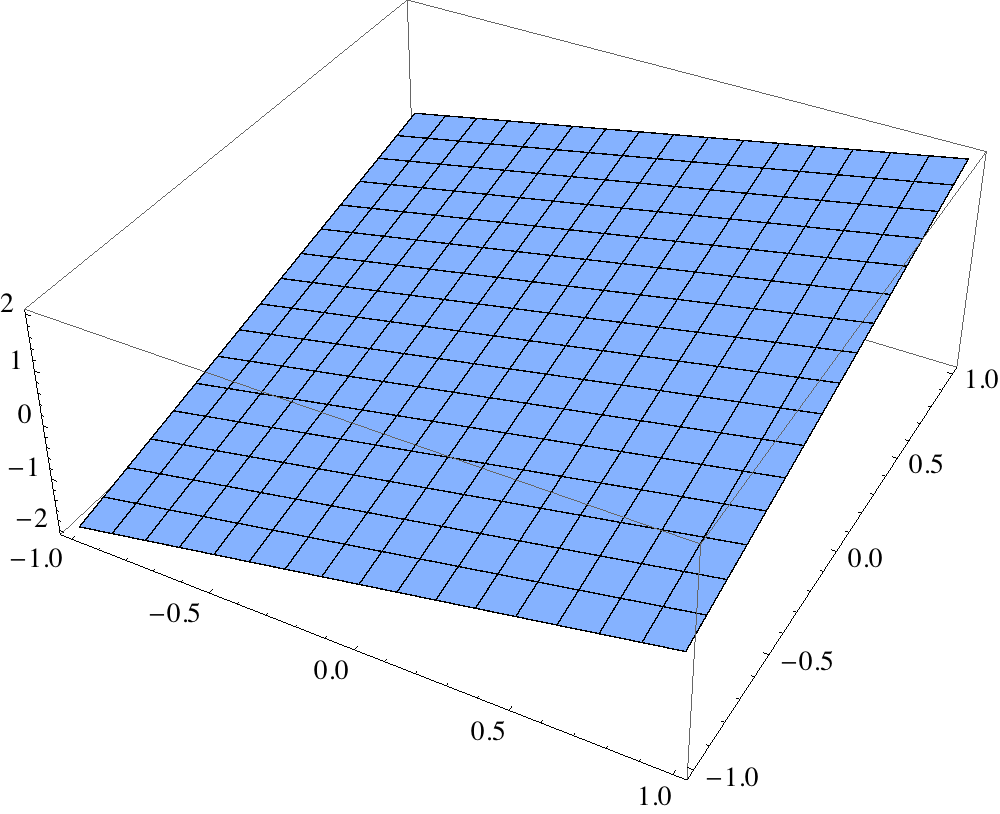
\includegraphics[width=0.35\textwidth]{pics/3ott/simplef1.png}\label{subfloat:3ott_1}}
  \hspace{0.5cm}
  \subfloat[][Level sets]{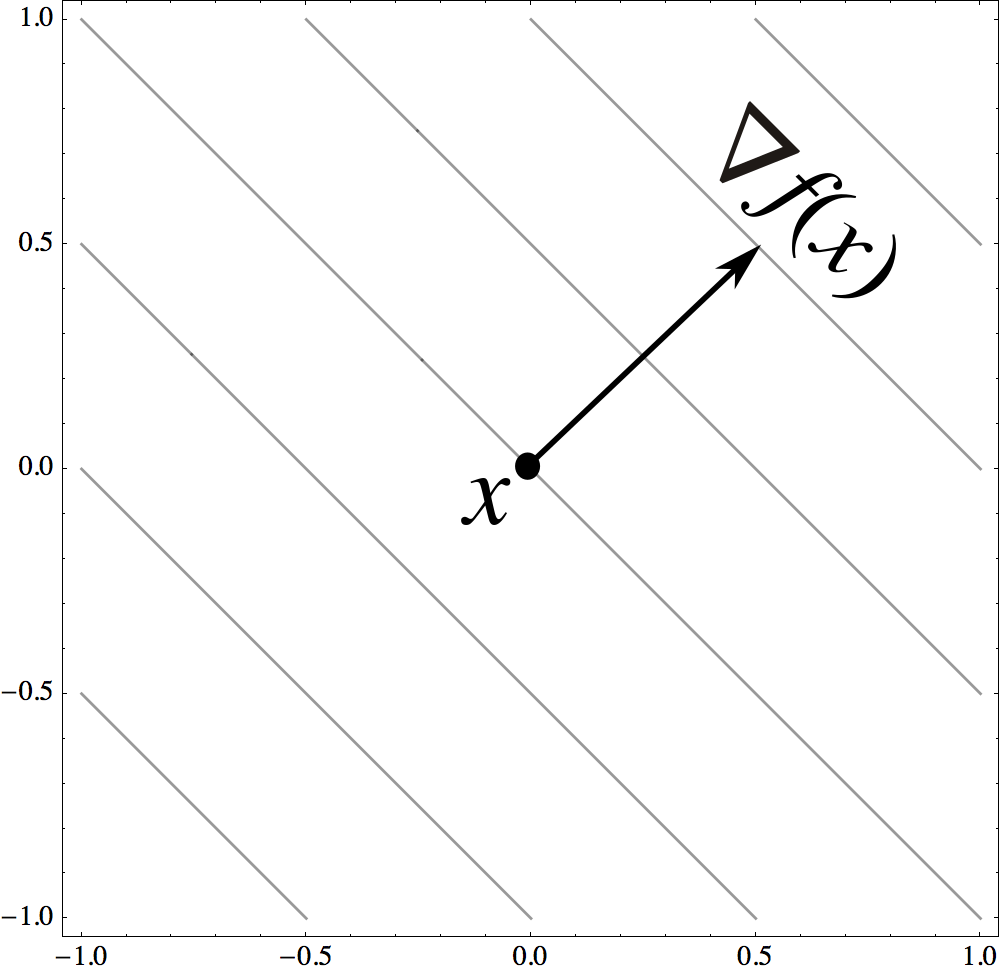
\includegraphics[width=0.29\textwidth]{pics/3ott/simplef2.png}\label{subfloat:3ott_2}}\\
  \caption{Graphical example of linear function.}\label{fig:3ott_1}
\end{figure}

\subsubsection{Quadratic functions}
Let us move to more interesting objects, aka quadratic functions: $f(x) = \frac{1}{2} x^T Q x + qx$, where $Q \in \R^{n\times n}$, $q \in \R^n$.

In \Cref{fig:3ott_2} we can see the plot of the quadratic function where 
\[
  Q = \left[\begin{array}{rr} 6 & -2 \\ -2 & 6 \end{array}\right]
  q = \left[\begin{array}{rr} 0 \\ 0 \end{array}\right]
\]

\begin{figure}[h]
  \centering
  \subfloat[][Quadratic function]{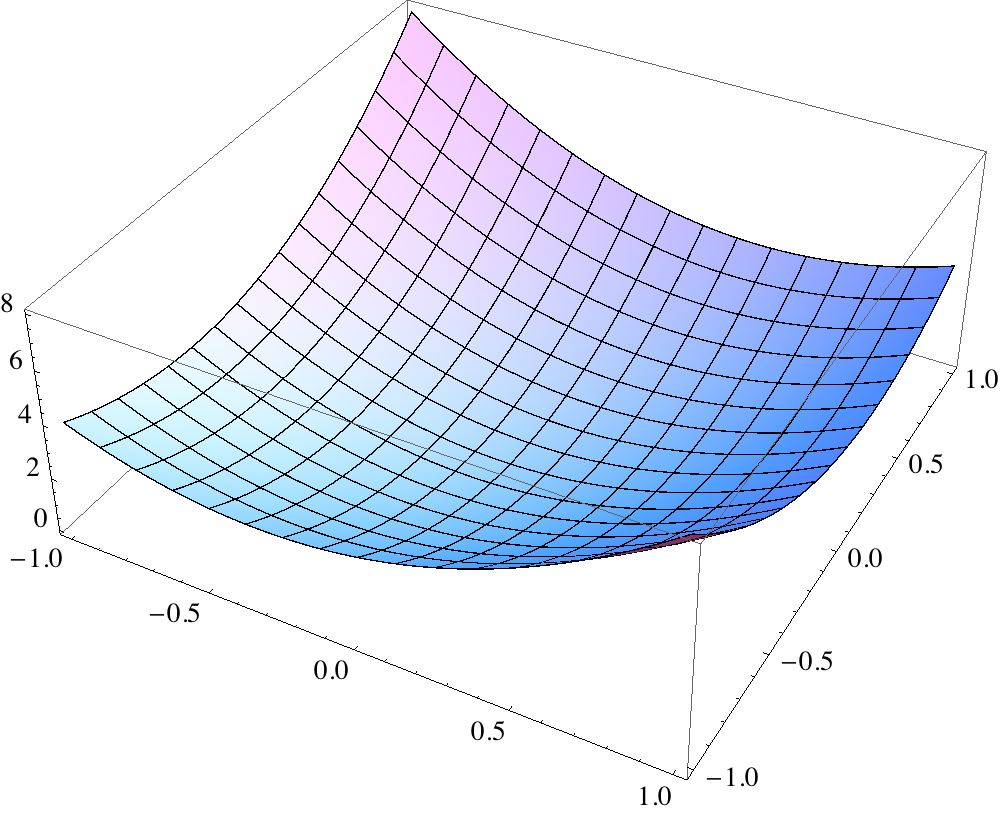
\includegraphics[width=0.35\textwidth]{pics/3ott/simplef3.png}\label{subfloat:3ott_3}}
  \hspace{0.5cm}
  \subfloat[][Level sets]{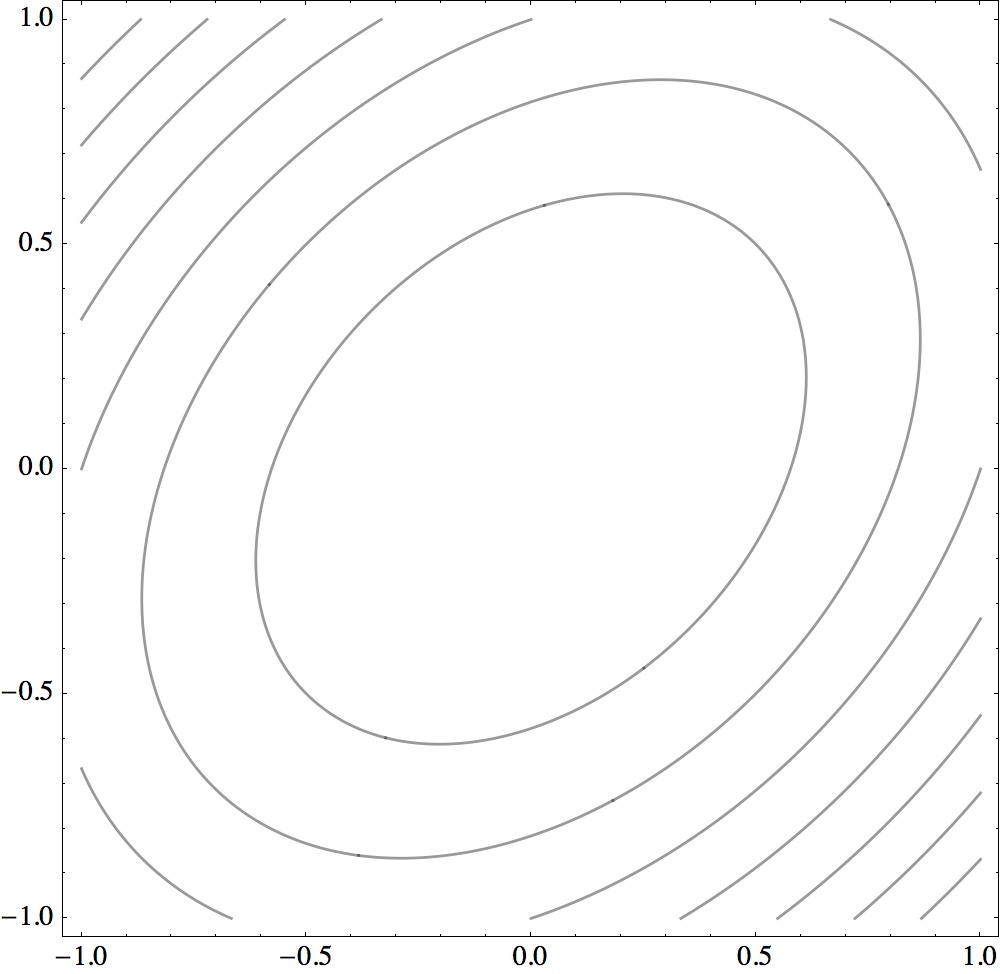
\includegraphics[width=0.29\textwidth]{pics/3ott/simplef4.png}\label{subfloat:3ott_4}}\\
  \caption{Graphical example of a quadratic function.}\label{fig:3ott_2}
\end{figure}

In quadratic functions the gradient is a linear function on $x$ ($\nabla f(x) = Q x + q$), while the Hessian is just $Q$ ($\nabla^2 f(x) = Q$) and the level sets are ellipsoids.
Sometimes such ellipses can degenerate to lines, in the case that one of the axis has become $+\infty$.

\begin{proposition}
  We can always assume that if $Q$ is symmetric, then it has spectral decomposition.
\end{proposition}

\begin{proof}
$x^T Q x = \frac{[(x^T Q x) + {(x^T Q x)}^T]}{2} = x^T [\frac{(Q + Q^T )}{2}] x = H \Lambda H^T$
\end{proof}

We will almost always assume that $Q$ is symmetric.

Let us consider the ``easy case'', where $Q$ is non singular (aka $\lambda_i \neq 0 \forall i$).

In this case,  $\bar{x} = - \inv{Q} q$, where $\bar{x}$ is called the center of the ellipsoid.
Let us assume that we moved the origin in such $\bar{x}$, so $y = x - \bar{x}$ and $f_{\bar{x}}(y) = \frac{1}{2} y^T Q y$.

\begin{proposition}
Along $H_i$: $f(\alpha) = f_{\bar{x}}( \alpha H_i ) = \alpha^2 \lambda_i$
\end{proposition}

Moreover, the size of the axes of the level curves is proportional to $\sqrt{1 / \lambda_i}$.
If the eigenvalues are $0$ then the axes get very long (but we would be in the case of $Q$ singular), on the other hand, if $\lambda_i < 0$, we no longer have axes.

\begin{proposition}
We can state the following:
\begin{itemize}
  \item $\forall i \, \lambda_i > 0 \equiv Q \succ 0 \Longrightarrow \bar{x}$ minimum of $f$;
  \item $\exists i \lambda_i < 0 \Longrightarrow f$ unbounded below.
\end{itemize}
\end{proposition}

\end{document}

